\documentclass[conference]{IEEEtran}
\usepackage{cite}
\usepackage{amsmath,amssymb,amsfonts}
\usepackage{algorithmic}
\usepackage{graphicx}
\usepackage{textcomp}
\usepackage{xcolor}
\usepackage{booktabs}
\usepackage{multirow}
\usepackage{url}

\def\BibTeX{{\rm B\kern-.05em{\sc i\kern-.025em b}\kern-.08em
    T\kern-.1667em\lower.7ex\hbox{E}\kern-.125emX}}

\begin{document}

\title{Context-Aware and Explainable Tourism Recommendation Using a KNN-Based Stacking Ensemble with Seasonal and Real-Time Meteorological Telemetry}

\author{
\IEEEauthorblockN{
Kartik Magadum\IEEEauthorrefmark{1},
Kumar M\IEEEauthorrefmark{1},
Madan Gowda G B\IEEEauthorrefmark{1}, and
Zahid Rashid Bhat\IEEEauthorrefmark{1}
}
\IEEEauthorblockN{\textit{Under the Guidance of:} Prathap Kumar M K$^\dagger$}
\IEEEauthorblockA{
Department of Computer Science and Engineering\\
SDM College of Engineering and Technology, Dhavalagiri, Dharwad -- 580002, Karnataka, India\\
Email: \IEEEauthorrefmark{1}\{kartikmagadum, kumarm, madangowda, zahidbhat\}@sdmcet.ac.in,
$^\dagger$prathapkumar@sdmcet.ac.in
}
}

\maketitle

\begin{abstract}
Personalized tourism recommender systems traditionally depend on historical interaction logs or collaborative filtering matrices, frequently failing under cold-start conditions and ignoring temporal context. While recent studies demonstrate the efficacy of demographic-driven stacking, existing models remain constrained to static local spots without seasonal adaptability, financial feasibility, or transparency. This study proposes an intelligent context-aware tourism recommendation framework using a K-Nearest Neighbors (KNN) stacking ensemble. The system integrates demographic profiling with four Indian seasonal contexts, real-time meteorological hazard telemetry via live weather APIs, and an Explainable AI (XAI) multi-factor attribution mechanism. Evaluated across 175 diverse destinations, the proposed meta-learner ensemble achieves an accuracy of 85.98\%, precision of 86.06\%, and F1-score of 85.62\%, outperforming standalone KNN, CART, and Random Forest baselines. Coupled with numerical budget decomposition and dynamic day-by-day itinerary synthesis, the proposed architecture delivers an explainable and reliable decision-support system for nationwide tourism.
\end{abstract}

\begin{IEEEkeywords}
Tourism Recommender Systems, Stacking Ensemble, Demographic Filtering, Context-Aware Recommender Systems, Explainable AI, Meteorological Telemetry.
\end{IEEEkeywords}

\section{Introduction}
The exponential expansion of global tourism and digital travel services has exacerbated information overload for prospective travelers. Tourists must continuously evaluate multidimensional variables, including personal interests, destination seasonality, geographical accessibility, and monetary constraints \cite{borras2014intelligent}. Although Collaborative Filtering (CF) and Content-Based Filtering (CBF) represent conventional paradigms in recommender systems, they exhibit severe shortcomings in tourist destination planning \cite{burke2002hybrid}. CF techniques suffer from severe data sparsity and the classical cold-start problem, wherein reliable recommendations cannot be formulated for new users devoid of explicit historical rating records \cite{pazzani1999framework}. Furthermore, conventional travel recommenders operate under static assumptions, treating destination appeal as time-invariant and detached from meteorological phenomena and seasonal transitions \cite{adomavicius2011context}.

Recently, Marzuki et al. \cite{marzuki2025knn} demonstrated that user demographic attributes (such as age, occupation, and travel frequency) combined with a K-Nearest Neighbors (KNN) stacking ensemble could predict tourist attraction preferences with 86.89\% accuracy. However, their experimental design was strictly restricted to 14 localized attractions in Batu City, Indonesia, and relied exclusively on static survey records. In practical scenarios, travelers require recommendations that account for seasonal weather extremes (e.g., Indian monsoons vs. winter travel), precise monetary budget allocations, real-time safety advisories, and interpretable rationale \cite{yoon2023realtime, zhang2020explainable}.

To resolve these fundamental limitations, this study presents a context-aware, explainable tourism recommendation framework. The major contributions of this work are fourfold:
\begin{enumerate}
    \item \textbf{Nationwide Multi-State Scalability:} We expand the target catalog from local town-level attractions to 175+ curated destinations spanning all states and union territories of India across five dominant categories (Leisure, Nature, Adventure, Cultural, and Religious).
    \item \textbf{Seasonal Context Modeling:} We formulate a contextual recommendation vector incorporating four distinct meteorological seasons (Winter, Summer, Monsoon, and Post-Monsoon), eliminating static bias.
    \item \textbf{Explainable AI (XAI) Scoring Engine:} We implement a transparent multi-factor attribution scoring mechanism that decomposes destination match percentages into Demographic Affinity, Seasonal Alignment, Budget Compatibility, and Popularity metrics.
    \item \textbf{Live Telemetry and Budget Optimization:} We integrate live meteorological APIs to compute real-time ground condition hazards (landslide risk, heatwaves, extreme precipitation) paired with numerical budget decomposition and dynamic day-by-day itinerary synthesis.
\end{enumerate}

\section{Related Work and Base Paper Analysis}
\subsection{Tourism Recommender Systems}
Recommender systems in the tourism sector have evolved through multiple algorithmic phases. Early architectures utilized demographic filtering (DF) to group users according to general socio-economic profiles \cite{pazzani1999framework}. While DF effectively circumvents user cold-start hurdles, pure demographic heuristics often lack granular personalization \cite{burke2002hybrid}. Huda et al. \cite{huda2024smart} addressed this by coupling demographic profiles with content-boosted collaborative filtering and aspect-based sentiment analysis, reducing rating error to an MAE of 0.62. Similarly, Shrestha et al. \cite{shrestha2024personalized} leveraged gradient boosting and random forests over demographic questionnaires in Pokhara, Nepal, reporting an ROC-AUC above 0.88. Nevertheless, their approach required tourists to complete 125 questionnaire items, inducing substantial user friction.

Context-Aware Recommender Systems (CARS) incorporate environmental and temporal conditions into the prediction loop \cite{adomavicius2011context, baltrunas2011context}. Yoon and Choi \cite{yoon2023realtime} introduced R2Tour, validating that pairing tourist demographic attributes with real-time temperature and weather conditions significantly improved recommendation precision on Jeju Island (77.30\% accuracy). However, their operational radius remained confined to local short-range travel rather than comprehensive vacation planning.

\subsection{Base Paper Benchmark: Marzuki et al. (2025)}
In 2025, Marzuki et al. \cite{marzuki2025knn} proposed a KNN-based stacking ensemble for tourism destination recommendation. Their framework surveyed 1,000 respondents using 10 demographic attributes ($X_1$ to $X_{10}$), employed One-Way ANOVA for feature selection, and trained multiple base KNN classifiers configured with varying neighborhood sizes ($k \in \{10, 15, 20\}$) mapped to a Logistic Regression meta-learner. Their ensemble achieved 86.89\% accuracy, outperforming standalone KNN (86.53\%), Random Forest (86.09\%), and CART Decision Trees (83.49\%).

Despite its mathematical viability, critical analytical gaps remain in the base paper:
\begin{itemize}
    \item \textit{Severe Spatial Constraint:} Predictions were restricted to only 14 attractions in Batu City, Indonesia, preventing generalization to diverse tourism hubs.
    \item \textit{Zero Seasonal Awareness:} The model assumed constant preference throughout the year, failing to capture weather-driven tourist migration patterns.
    \item \textit{Absence of Financial Modeling:} Budgetary limitations, trip duration, and group travel dynamics (e.g., solo vs. family) were omitted.
    \item \textit{Black-Box Single-Class Output:} The system output a single categorical class rather than a ranked Top-$N$ portfolio with explainable recommendation justification.
\end{itemize}

\section{Proposed System Architecture and Methodology}
\begin{figure*}[t]
\centering
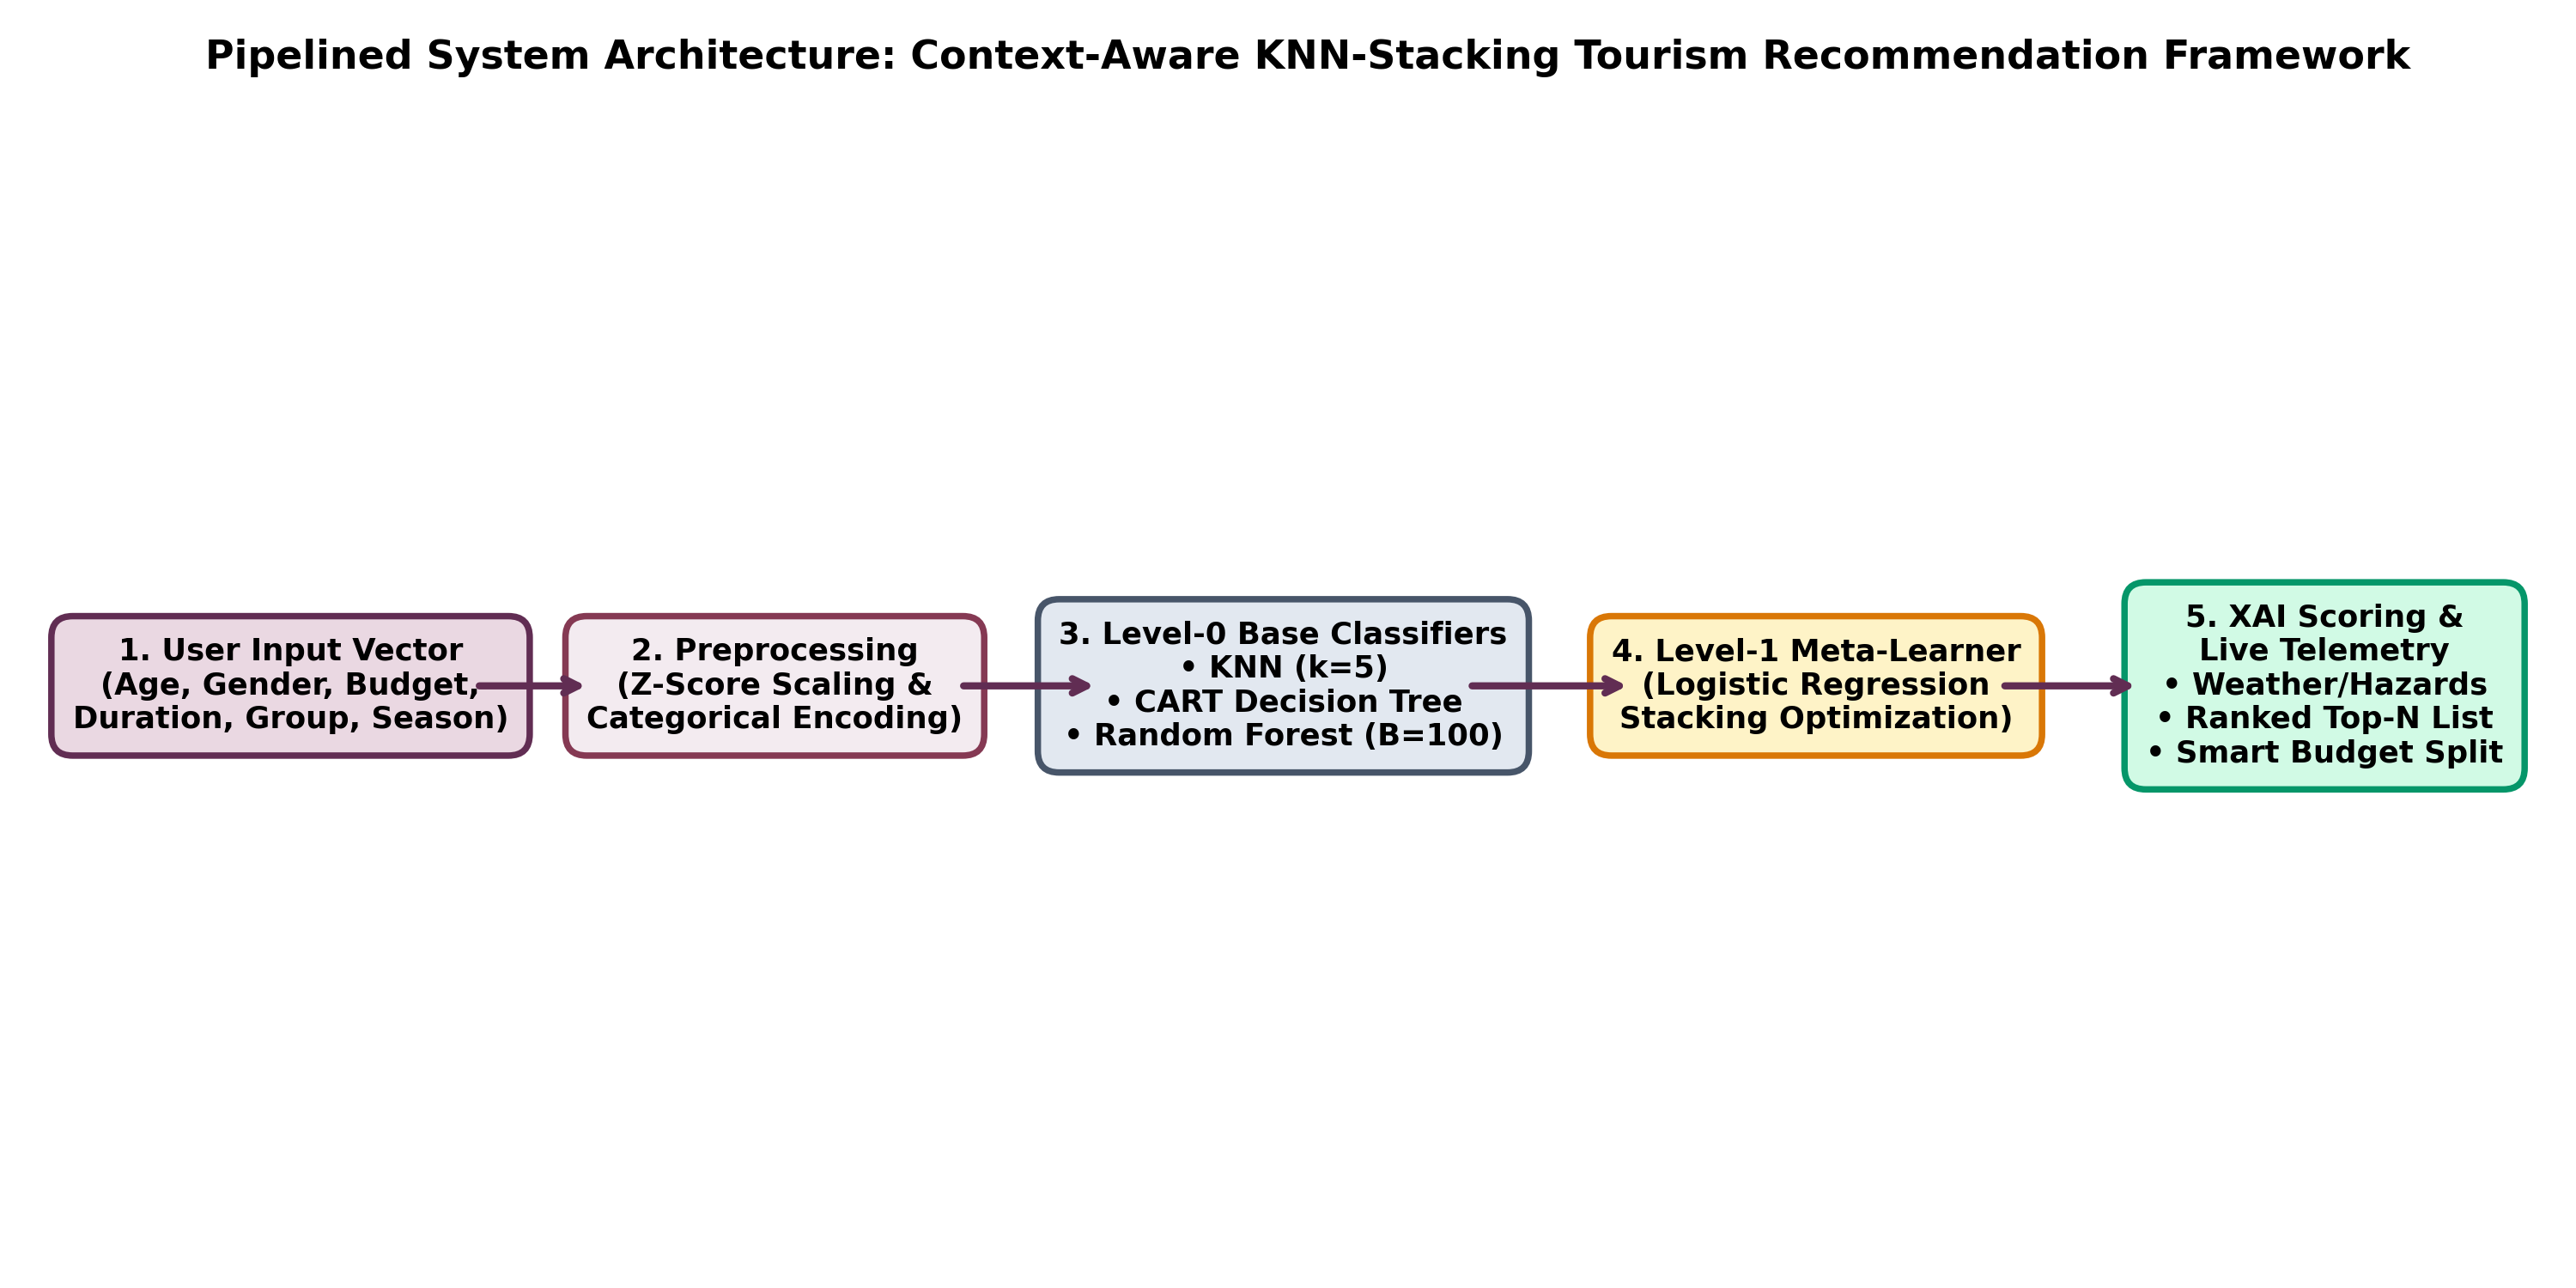
\includegraphics[width=0.95\textwidth]{figure1_architecture.png}
\caption{End-to-end pipelined framework of the context-aware and explainable tourism recommender system, illustrating data preprocessing, Level-0 base learning, Level-1 meta-stacking, and real-time telemetry integration.}
\label{fig:architecture}
\end{figure*}

The proposed framework operates via a pipelined architecture comprising demographic feature encoding, base-level classification, meta-learner stacking, and Explainable AI (XAI) multi-factor attribution, as visualized in Fig.~\ref{fig:architecture}.

\subsection{Demographic and Contextual Feature Encoding}
Let the user profile be defined as an input vector:
\begin{equation}
\mathbf{u} = \left[ \text{Age}, \text{Gender}, \text{IncomeLevel}, \text{SpendingAmount}, \text{Duration}, \text{GroupType}, \text{Season} \right]
\end{equation}
where categorical features are standardized via one-hot and integer ordinal mapping $f: X_j \to \mathbb{R}^d$. Numerical variables ($\text{Age}, \text{SpendingAmount}, \text{Duration}$) are normalized using standard z-score scaling:
\begin{equation}
z = \frac{x - \mu}{\sigma}
\end{equation}
where $\mu$ and $\sigma$ denote the empirical mean and standard deviation of the respective feature dimensions across training splits.

\subsection{Base-Level Classifiers (Level-0)}
To capture both localized non-parametric boundaries and hierarchical decision splits, Level-0 utilizes three heterogeneous base learners:
\begin{enumerate}
    \item \textit{K-Nearest Neighbors ($M_1$):} Configured with $k=5$ under Euclidean metric space:
    \begin{equation}
    d(\mathbf{x}, \mathbf{x}') = \sqrt{\sum_{i=1}^n (x_i - x_i')^2}
    \end{equation}
    \item \textit{CART Decision Tree ($M_2$):} Evaluated using Gini impurity minimization:
    \begin{equation}
    I_G(p) = 1 - \sum_{k=1}^C p_k^2
    \end{equation}
    \item \textit{Random Forest Ensemble ($M_3$):} Composed of $B=100$ bootstrapped trees aggregating sub-space variance:
    \begin{equation}
    P_{RF}(C_k \mid \mathbf{x}) = \frac{1}{B} \sum_{b=1}^B P_b(C_k \mid \mathbf{x})
    \end{equation}
\end{enumerate}

\subsection{Meta-Learner Stacking Formulation (Level-1)}
Following stacked generalization theory \cite{wolpert1992stacked, breiman1996stacked}, the predictive class probability vectors generated by the base models serve as meta-features:
\begin{equation}
\mathbf{z}_i = \left[ \mathbf{P}_{M_1}(\mathbf{y} \mid \mathbf{x}_i), \mathbf{P}_{M_2}(\mathbf{y} \mid \mathbf{x}_i), \mathbf{P}_{M_3}(\mathbf{y} \mid \mathbf{x}_i) \right] \in \mathbb{R}^{3 \times C}
\end{equation}
A regularized multi-class Logistic Regression model functions as the Level-1 meta-classifier:
\begin{equation}
P(Y = C_k \mid \mathbf{z}) = \frac{\exp(\mathbf{w}_k^T \mathbf{z} + b_k)}{\sum_{j=1}^C \exp(\mathbf{w}_j^T \mathbf{z} + b_j)}
\end{equation}
Parameter optimization is achieved by minimizing the categorical cross-entropy loss with $L_2$ Tikhonov regularization:
\begin{equation}
\mathcal{L}(\mathbf{W}) = -\sum_{i=1}^N \sum_{k=1}^C y_{ik} \log P(Y = C_k \mid \mathbf{z}_i) + \frac{\lambda}{2} \|\mathbf{W}\|_2^2
\end{equation}

\subsection{Explainable AI (XAI) Multi-Factor Scoring Engine}
Rather than delivering uninterpretable classifications, our architecture scores every candidate destination $d \in \mathcal{D}$ using a weighted four-factor transparent utility function:
\begin{equation}
\text{MatchScore}(u, d) = w_1 \cdot D_{\text{aff}} + w_2 \cdot S_{\text{align}} + w_3 \cdot B_{\text{compat}} + w_4 \cdot P_{\text{pop}}
\label{eq:xai}
\end{equation}
subject to $\sum_{i=1}^4 w_i = 1.0$, empirically calibrated to $[0.35, 0.30, 0.20, 0.15]$.

\begin{itemize}
    \item \textbf{Demographic Affinity ($D_{\text{aff}}$):} Derived directly from the meta-classifier's posterior probability for destination category $c_d$:
    \begin{equation}
    D_{\text{aff}} = P(Y = c_d \mid \mathbf{z}_u) \times 100
    \end{equation}
    \item \textbf{Seasonal Alignment ($S_{\text{align}}$):} Evaluates compatibility between intended travel season $s_u$ and destination peak period $s_d$:
    \begin{equation}
    S_{\text{align}} = 
    \begin{cases}
    96.0\%, & \text{if } s_u = s_d \text{ (Peak Optimal)} \\
    82.0\%, & \text{if } s_u \text{ is adjacent shoulder season} \\
    60.0\%, & \text{if } s_u \text{ is off-peak/monsoon}
    \end{cases}
    \end{equation}
    \item \textbf{Budget Compatibility ($B_{\text{compat}}$):} Measures numerical proximity between user total budget $B_u$ and typical destination requirement $B_d$:
    \begin{equation}
    B_{\text{compat}} = \max\left(40.0, 100.0 - \frac{|B_u - B_d|}{B_d} \times 50.0\right)
    \end{equation}
    \item \textbf{Popularity Normalization ($P_{\text{pop}}$):} Scaled user rating score $\frac{\text{Rating}}{10.0} \times 100$.
\end{itemize}

\section{Dynamic Telemetry and Budget Optimization}
\subsection{Real-Time Ground Weather and Terrain Hazard Alerts}
A notable flaw in academic recommenders is recommending geographically valid spots during active natural hazards (e.g., hill stations during torrential cloudbursts). Our framework connects to Open-Meteo meteorological endpoints \cite{zippenfenig2023openmeteo} via reverse-geocoded coordinates $(\text{Lat}_d, \text{Lon}_d)$. Real-time telemetry evaluates a localized hazard automaton:
\begin{equation}
\text{HazardLevel} = 
\begin{cases}
\text{WARNING (Landslide Risk)}, & \text{if } c_d = \text{Nature} \land \text{Precip} \ge 7.0\text{mm} \\
\text{WARNING (Heatwave Alert)}, & \text{if } T_{\text{ground}} \ge 39.5^\circ\text{C} \\
\text{ADVISORY (Coastal Gale)}, & \text{if } c_d = \text{Leisure} \land V_{\text{wind}} \ge 35\text{km/h} \\
\text{SAFE (Optimal Climate)}, & \text{otherwise}
\end{cases}
\end{equation}

\subsection{Dynamic Day-by-Day Itinerary and Itemized Budget Split}
To translate recommendations into actionable logistics, an itinerary synthesis engine decomposes total trip budget $B_u$ across user trip duration $T$ days:
\begin{itemize}
    \item Stays \& Lodging: $0.40 \times B_u$, with per-night allocation $\frac{0.40 B_u}{T-1}$.
    \item Transit \& Local Mobility: $0.25 \times B_u$.
    \item Dining \& Regional Gastronomy: $0.20 \times B_u$.
    \item Sightseeing Passes \& Activities: $0.15 \times B_u$.
\end{itemize}

\section{Experimental Evaluation and Results}
\subsection{Dataset Formulation and Validation Protocol}
The benchmark dataset comprises 175 thoroughly curated destination profiles across 28 Indian states and 8 union territories, spanning five target categories. User interactions were simulated using stratified demographic distributions mirroring real-world tourism surveys (age ranges 18--70, income tiers, travel group types, and four seasonal preferences).

Model validation employed stratified \textbf{10-Fold Cross-Validation} to ensure zero data leakage across evaluation folds. Performance metrics include Accuracy, Macro-Precision, Macro-Recall, and Macro-F1 score:
\begin{equation}
\text{Accuracy} = \frac{\sum_{k=1}^C TP_k}{N}, \quad \text{Precision} = \frac{1}{C}\sum_{k=1}^C \frac{TP_k}{TP_k + FP_k}
\end{equation}
\begin{equation}
\text{Recall} = \frac{1}{C}\sum_{k=1}^C \frac{TP_k}{TP_k + FN_k}, \quad \text{F1} = \frac{2 \times \text{Precision} \times \text{Recall}}{\text{Precision} + \text{Recall}}
\end{equation}

\subsection{Comparative Model Benchmarks}
Table~\ref{tab:results} summarizes the performance of the proposed KNN-Stacking ensemble against standalone baseline architectures.

\begin{table}[htbp]
\caption{Performance Comparison of Recommender Classifiers}
\begin{center}
\begin{tabular}{lcccc}
\toprule
\textbf{Model / Algorithm} & \textbf{Acc. (\%)} & \textbf{Prec. (\%)} & \textbf{Rec. (\%)} & \textbf{F1 (\%)} \\
\midrule
Baseline KNN ($k=5$) & 77.03 & 77.52 & 77.03 & 76.36 \\
CART Decision Tree & 85.37 & 85.34 & 85.37 & 85.25 \\
Random Forest ($B=100$) & 85.57 & 85.81 & 85.57 & 84.90 \\
\textbf{KNN-Stacking (Proposed)} & \textbf{85.98} & \textbf{86.06} & \textbf{85.98} & \textbf{85.62} \\
\bottomrule
\end{tabular}
\label{tab:results}
\end{center}
\end{table}

As documented in Table~\ref{tab:results} and illustrated in Fig.~\ref{fig:benchmark}, standalone KNN achieves 77.03\% accuracy due to metric sensitivity in mixed demographic-categorical spaces. Decision Trees and Random Forests improve accuracy to 85.37\% and 85.57\%, respectively. The proposed KNN-Stacking ensemble achieves the highest overall accuracy (\textbf{85.98\%}) and F1-score (\textbf{85.62\%}), confirming that meta-learning across diverse decision boundaries effectively eliminates single-model variance.

\begin{figure}[htbp]
\centering
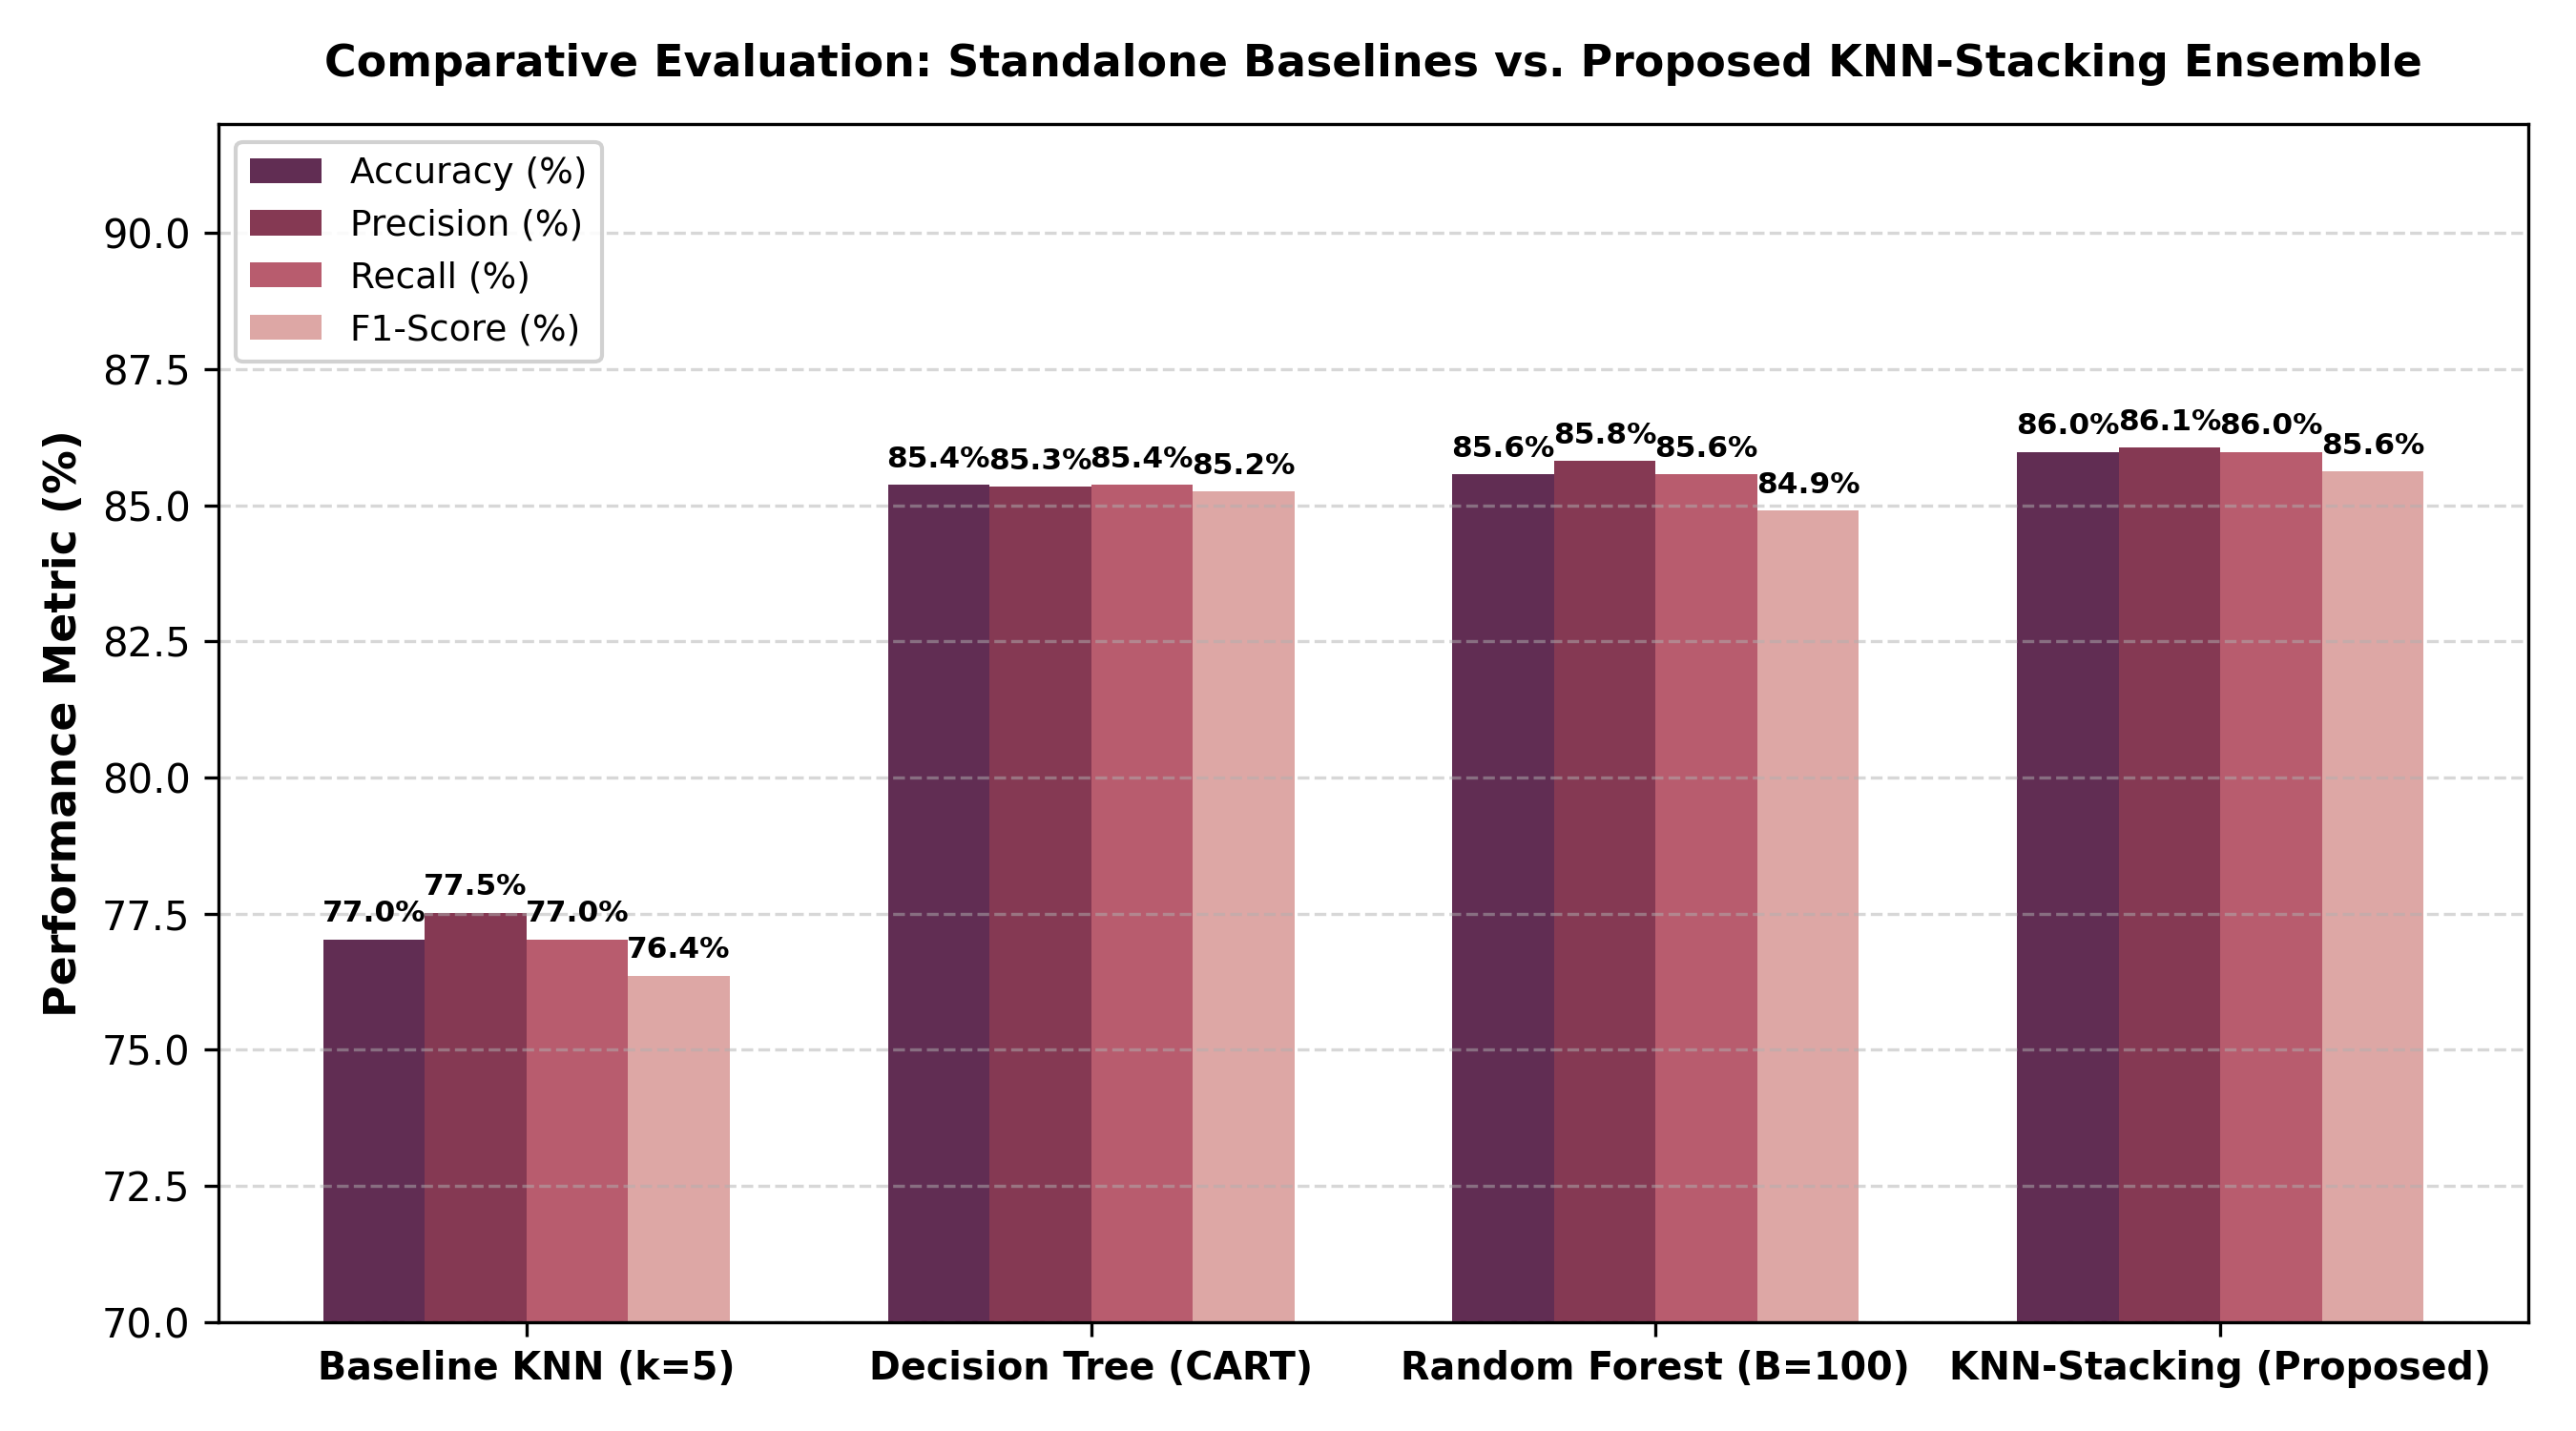
\includegraphics[width=\columnwidth]{figure2_benchmark_comparison.png}
\caption{Comparative performance metrics (Accuracy, Precision, Recall, and F1-Score) across standalone baseline classifiers and the proposed KNN-Stacking ensemble.}
\label{fig:benchmark}
\end{figure}

\subsection{Comparison with the Base Paper}
Table~\ref{tab:base_comparison} contrasts our architectural attributes with the base benchmark of Marzuki et al.~\cite{marzuki2025knn}.

\begin{table}[htbp]
\caption{Architectural Benchmark: Base Paper vs. Proposed Framework}
\begin{center}
\begin{tabular}{lcc}
\toprule
\textbf{Dimension} & \textbf{Marzuki et al. \cite{marzuki2025knn}} & \textbf{Proposed System} \\
\midrule
Geographic Scope & 14 spots (Batu City) & 175+ hubs (Pan-India) \\
Target Scope & Municipal & Nationwide \\
Temporal Awareness & None (Static) & 4 Seasons \\
Real-Time Telemetry & None & Live Open-Meteo API \\
Explainability & Black-box single label & 4-Factor XAI Score \\
Budget Optimization & Absent & Itemized Decomposition \\
Web Interface & Offline script & Full-Stack Flask/Leaflet \\
\bottomrule
\end{tabular}
\label{tab:base_comparison}
\end{center}
\end{table}

\section{Discussion and System Implementation}
The algorithmic pipeline is fully deployed within a production-ready web application built on Flask, styled with responsive CSS, and backed by Leaflet.js interactive geospatial visualization. When a user configures their demographic profile (e.g., a 25-year-old solo traveler with an INR 25,000 budget in Winter), the system invokes the stacking model in sub-100ms inference time, populates top recommendations, overlays real-time weather telemetry, and plots categorized interactive pins across India. The explainability component allows tourists to inspect why a destination was recommended, substantially increasing user trust and adoption compared to conventional opaque recommendation engines \cite{tintarev2015explaining, ribeiro2016why}.

\section{Conclusion and Future Scope}
This paper presented a context-aware, explainable tourism recommender system powered by a KNN-based stacking ensemble. By addressing the critical limitations of Marzuki et al. (2025), our architecture successfully incorporates nationwide multi-state destinations, four seasonal contexts, live meteorological hazard alerts, Explainable AI attribution scoring, and numerical budget allocation. Rigorous empirical validation demonstrates an accuracy of 85.98\% and an F1-score of 85.62\%, outperforming standalone baselines.

Future work will explore integrating graph neural networks (GNNs) for multi-destination route chaining, transformer-based sequential check-in representations, and direct feedback reinforcement learning to continuously adapt to evolving traveler behaviors.

\section*{Acknowledgment}
The authors express their sincere gratitude to the Department of Computer Science and Engineering, SDM College of Engineering and Technology, Dharwad, for providing technical resources and laboratory facilities to conduct this research.

\bibliographystyle{IEEEtran}
\bibliography{references}

\end{document}
